\documentclass[12pt,a4paper]{article}
\usepackage{amsfonts, amssymb, amsmath}
\usepackage{fullpage}
\usepackage{parskip} % skip a line instead of indenting
\usepackage{amsthm}
\usepackage{xcolor}
\usepackage{tikz}

\newtheorem*{rem}{Remark}

\title{Vector Spaces and Subspaces}
\author{R4 Cheng}
\date{\today}

\newcommand{\Remark}[1]{
  \begin{rem}
    \color{cyan}
    #1
  \end{rem}
}

\begin{document}
\maketitle

$\mathbb{R}^n = $ all (column) vectors with n (real) components. \\
$= \{ (v_1, v_2, \cdots, v_n): v_i \in \mathbb{R}, i = 1, 2, \cdots, n \}$

\[
\begin{bmatrix}
  4 \\
  \pi \\
\end{bmatrix} \in \mathbb{R}^2,
\quad
(1, 1, 0, 1, 1) \in \mathbb{R}^5
\]
\[
\begin{tikzpicture}
  % Draw x-axis
  \draw[->] (-2, 0) -- (2, 0) node[right] {$x$};
  % Draw y-axis
  \draw[->] (0, -2) -- (0, 2) node[above] {$y$};
  
  % Draw vector v
  \draw[->, red] (0, 0) -- (1, 1) node[midway, below right] {$\mathbf{v}$};
  \draw[->, pink] (0, 0) -- (3, 3) node[midway, above right] {$\mathbf{3v}$};
  
  % Draw vector w
  \draw[->, blue] (0, 0) -- (1, 2) node[midway, above left] {$\mathbf{w}$};
  
  % Draw vector v + vector w
  \draw[->, purple] (0, 0) -- (2, 3) node[above right] {$\mathbf{v} + \mathbf{w}$};
\end{tikzpicture}
\]

\subsection*{Vector Space $V$}

$V$: a set of vectors
\begin{enumerate}
  \item Two operations:
  \begin{itemize}
    \item vector addition: $\underline{v}, \underline{w} \in V \Rightarrow \underline{v} + \underline{w} \in V$
    \item scalar multiplication: $c \underline{v} \in V$
  \end{itemize}
  \item Eight rules:
  \begin{enumerate}
    \item $\underline{v} + \underline{w} = \underline{w} + \underline{v}$ (commutative)
    \item $(\underline{v} + \underline{w}) + \underline{z} = \underline{v} + (\underline{w} + \underline{z})$ (associative)
    \item There is a unique "zero vector" \underline{0} such that $\underline{v} + \underline{0} = \underline{v}$ for all $\underline{v} \in V$
    \item For each $\underline{v}$, there is a unique vector $-\underline{v}$ such that $\underline{v} + (-\underline{v}) = \underline{0}$
    \item $1 \times \underline{v} = \underline{v}$
    \item $(c_1c_2)\underline{v} = c_1(c_2\underline{v})$
    \item $c(\underline{v} + \underline{w}) = c\underline{v} + c\underline{w}$
    \item $(c_1 + c_2)\underline{v} = c_1\underline{v} + c_2\underline{v}$
  \end{enumerate}
\end{enumerate}

$\Rightarrow 0 \times \underline{v}  = \underline{0}$  (not 0) \\
$\Rightarrow (-1)\underline{v} = -\underline{v}$

Example:

\begin{itemize}
  \item $\mathbb{R}^n$ is a vector space
  \item $M =$ \{all real $2 \times 2$ matrices\} is a vector space
  \item $F =$ \{all real functions $f(x)$ \} is a vector space
  \item $z = \{ \underline{0} \}$ is a vector space
\end{itemize}

\subsection*{Subspaces}

\textbf{Def.} A subset W of a vector space V is a \underline{subspaces} if W itself is a vector space.

Check:

\begin{itemize}
  \item $\underline{v}, \underline{w} \in W \Rightarrow \underline{v} + \underline{w} \in W$
  \item $\underline{v} \in W, c\underline{v} \in W$ for any $c$
\end{itemize}

\textbf{Claim} Every subspace contains the zero vector.

\textbf{Proof} TODO

Example:

1. 

$U = \{(x, y): x \geq 0, y \geq 0\}$, is $U$ a subspace?
$
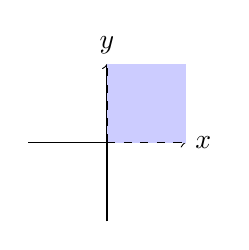
\begin{tikzpicture}
  % Draw x-axis
  \draw[->] (-1, 0) -- (1, 0) node[right] {$x$};
  % Draw y-axis
  \draw[->] (0, -1) -- (0, 1) node[above] {$y$};

  % Shade the first quadrant
  \fill[color=blue!20] (0,0) rectangle (1,1);
    
  % Draw dashed lines along the boundaries
  \draw[dashed] (0,0) -- (1,0);
  \draw[dashed] (0,0) -- (0,1);
\end{tikzpicture}
$

No, since $-1(1, 0) = (-1, 0) \notin U$ even of $(1, 0) \in U$.

2.

$M =$ \{all real $2 \times 2$ matrices\} \\
$
\{
  U = 
  \begin{bmatrix}
    a & b \\
    0 & d \\
  \end{bmatrix}:
  a,\,b,\,d \in \mathbb{R}
\}
$

$A, B \in U$, $A + B \in U$ and $cA \in U$

$\therefore U$ is a subspace of $M$ 

\subsection*{Column Space}

\textbf{Def.} The column space $C(A)$ of a matrix $A$ consists of all linear combinations of the columns of $A$.

\Remark{C(A): C of A}

Example:

\[
  A = 
  \begin{bmatrix}
    1 & 0 \\
    4 & 3 \\
    2 & 3
  \end{bmatrix}
\]
\[
C(A) = \
\{
  c_1
  \begin{bmatrix}
    1 \\
    4 \\
    2
  \end{bmatrix}
  + c_2
  \begin{bmatrix}
    0 \\
    3 \\
    3
  \end{bmatrix}
  : c_1, c_2 \in \mathbb{R}
\}
\]
\[
= 
\{
  A\underline{c}: \underline{c} = 
  \begin{bmatrix}
    c_1 \\
    c_2
  \end{bmatrix} \in \mathbb{R}^2
\} (A\underline{x} = \underline{b})
\]

The set of all $A\underline{x}$ for all $x$ is called the column space.

$$\iff c_1[\underline{a_1}] + c_2[\underline{a_2}] + \cdots + c_n[\underline{a_n}]  = \underline{b}$$
$\therefore$ The system $A\underline{x} = \underline{b}$ is solvable iff $\underline{b} \in C(A)$

Example:

What are the column spaces of 1. $I$, 2.
$
A = 
\begin{bmatrix}
  1 & 2 \\
  2 & 4
\end{bmatrix}
$, 
3. 
$
B = 
\begin{bmatrix}
  1 & 2 & 3 \\
  0 & 0 & 4
\end{bmatrix}
$?

1. 

$
x_1
\begin{bmatrix}
  1 \\
  0
\end{bmatrix} + 
x_2
\begin{bmatrix}
  0 \\
  1
\end{bmatrix} = 
\begin{bmatrix}
  x_1 \\
  x_2
\end{bmatrix} \in \mathbb{R}^2
\therefore C(I) = \mathbb{R}^2
$

2.

$
x_1
\begin{bmatrix}
  1 \\
  2
\end{bmatrix} + 
x_2
\begin{bmatrix}
  2 \\
  4
\end{bmatrix} = 
x_1
\begin{bmatrix}
  1 \\
  2
\end{bmatrix} + 
2x_2
\begin{bmatrix}
  1 \\
  2
\end{bmatrix} =
(x_1 + 2x_2)
\begin{bmatrix}
  1 \\
  2
\end{bmatrix} \in \mathbb{R}^2 \Rightarrow
x_{real}
\begin{bmatrix}
  1 \\
  2
\end{bmatrix}
$

$\therefore C(A) =
\{
  x
  \begin{bmatrix}
    1 \\
    2
  \end{bmatrix}
  : x \in \mathbb{R}
\}
$

3.

$
x_1
\begin{bmatrix}
  1 \\
  0
\end{bmatrix} +
x_2
\begin{bmatrix}
  2 \\
  0
\end{bmatrix} +
x_3
\begin{bmatrix}
  3 \\
  4
\end{bmatrix} =
(x_1 + 2x_2 (= x_4))
\begin{bmatrix}
  1 \\
  0
\end{bmatrix} +
x_3
\begin{bmatrix}
  3 \\
  4
\end{bmatrix} 
$
$
  \begin{bmatrix}
    1 & 3 \\
    0 & 4
  \end{bmatrix}
  \begin{bmatrix}
    x_4 \\
    x_3
  \end{bmatrix} = 
  \begin{bmatrix}
    b_1 \\
    b_2
  \end{bmatrix}
$ is always solvable for any $b_1$, $b_2$

$
\because
\begin{bmatrix}
  1 & 3 \\
  0 & 4
\end{bmatrix}
$ is upper triangular matrix ($b_1$, $b_2$ must be found)
$\therefore C(B) = \mathbb{R}^2$

$\Rightarrow$ All of them are subspaces of $\mathbb{R}^2$

\textbf{Claim} If A is an $m \times n$ real matrix, then $C(A)$ is a subspace of $\mathbb{R}^m$

\textbf{Proof.} TODO

$S = $ the set of vectors in a vector space V (probably not a subspace) \\
$SS =$ the set of all linear combinations of vectors in S

We call $SS$ the "span" of $S$.

Then $SS$ is a subspace of $V$, called the subspace ``spanned'' by $S$.

E.g.

$S$ = the set of columns of 
$
A = 
\begin{bmatrix}
  1 & 2 \\
  2 & 3
\end{bmatrix}
$

$SS = $ the column space of $A = C(A)$

\subsection*{Null Space of $A$}

$$N(A) = \{\underline{x}: A\underline{x} = \underline{0}\}$$

\Remark{related to the "rank"}

\textbf{Claim} If $A$ is $m \times n$, then $N(A)$ is a subspace of $\mathbb{R}^n$.

\textbf{Proof} TODO

Example:
$
C = 
\begin{bmatrix}
  1 & 2 & 2 & 4 \\
  3 & 8 & 6 & 16 \\
\end{bmatrix} = [A \quad 2A]
$ (Two equations in four unknowns)

TODO

\[
  N(C) = \{ \underline{x}: \underline{x} = 
    x_3
    \begin{bmatrix}
      -2 \\
      0 \\
      1 \\
      0
    \end{bmatrix} + 
    x_4
    \begin{bmatrix}
      -2 \\
      0 \\
      1 \\
      0
    \end{bmatrix},\, x_3, x_4 \in \mathbb{R}
  \} 
\]

\Remark{Reduced Row Echelon form (RRE form) 1. Produce 0 above/below pivots 2. Produce 1 in pivots} 

Example:
$
A = 
\begin{bmatrix}
  1 & 1 & 2 & 3 \\
  2 & 2 & 8 & 10 \\
  3 & 3 & 10 & 13 \\
\end{bmatrix}
$

TODO

\[
  N(A) = \{ \underline{x}: \underline{x} = 
    x_2
    \begin{bmatrix}
      -1 \\
      1 \\
      0 \\
      0
    \end{bmatrix} + 
    x_4
    \begin{bmatrix}
      -1 \\
      0 \\
      -1 \\
      1
    \end{bmatrix},\, x_2, x_4 \in \mathbb{R}
  \} 
\]

Suppose $A$ is $m \times n$. If there are $r$ pivots ($r \leq m, n$),
there are $(n - r)$ free variables. And there are $(n - r)$ special solutions.
$N(A)$ consists of all the linear combinations of these $(n-r)$ special solutions.

\begin{center}
  $N(A) =$ the subspace spanned by these $(n-r)$ special solutions.
\end{center}

\textbf{Def.} The \textcolor{red}{rank} of a matrix $A$ is the number of pivots.

\Remark{All free columns are linear combinations of the pivot columns, and special solutions describe these combinations.}

\subsection*{Complete Solution to $A\underline{x} = \underline{b}$}

\[ \underline{x} = \underline{x}_{particular} + \underline{x}_{nullspace} \]

\textbf{Claim} If $A\underline{x}=\underline{b}$, 
then the complete solution is $\underline{x} = \underline{x}_{particular} + \underline{x}_{nullspace}$, 
where $\underline{x}_{particular}$ is a particular solution to $A\underline{x}=\underline{b}$, and $\underline{x}_{nullspace}$ is a general solution to $A\underline{x} = \underline{0}$.

\textbf{Proof} 

1. If $\underline{x} = \underline{x}_{particular} + \underline{x}_{nullspace}$, then 
$A\underline{x} = A(\underline{x}_{particular} + \underline{x}_{nullspace}) = A\underline{x}_{particular} + A\underline{x}_{nullspace} = \underline{b} + \underline{0} = \underline{b}$

$\therefore \underline{x}$ is a solution to $A\underline{x} = \underline{b}$

2. If $\underline{x}$ is a solution to $A\underline{x} = \underline{b}$, then
$A(\underline{x} - \underline{x}_p) = A\underline{x} - A\underline{x}_p = \underline{b} - \underline{b} = \underline{0}$

$\therefore \underline{x} - \underline{x}_p = \underline{x}_n$ is a solution to $A\underline{x} = \underline{0} \Rightarrow \underline{x} = \underline{x}_p + \underline{x}_n$

\fbox{
  \parbox{\linewidth}{
    \textbf{Q.} Suppose $A$ is a square invertible matrix ($m = n = pivots$). What are $\underline{x}_p$ and $\underline{x}_n$?

    \textbf{A.}

    The only particular solution to $A\underline{x} = \underline{b}$ is $\underline{x}_p = A^{-1}\underline{b}$. (because it is invertible)

    The only solution to $A\underline{x} = \underline{0}$ is $\underline{x}_n = \underline{0}$ (Inverse matrix's attribute).
  }
}

\textbf{Example: Full Column Rank}

TODO

In general, if $r = n (m\geq n)$ (A has full column rank), 

\[
A = [Matrix]_{m \times n}\ 
\Rightarrow 
R = 
\begin{bmatrix}
  I \\
  0
\end{bmatrix}
\]

Therefore, if $A$ has full column rank $(r=n)$, then 
\begin{enumerate}
  \item All columns of $A$ are pivot columns
  \item There are no free variables or no special solutions
  \item $N(a) = {\underline{0}}$
  \item If $A\underline{x} = \underline{b}$ is solvable, then the solution is unique.
\end{enumerate}

\textbf{Example: Full Row Rank}

TODO

In general, if $r = m (m\leq n)$ (A has full row rank), 

\[A = [Matrix]_{m \times n}\ \Rightarrow R = [I \quad F] \]

Therefore, if $A$ has full row rank $(r=m)$, then 
\begin{enumerate}
  \item All rows of $A$ are pivot columns and $R$ has no zero rows
  \item $A\underline{x} = \underline{b}$ is solvable for all $\underline{b}$
  \item $C(A) = \mathbb{R}^m$ ($C$: column space)
  \item There are $n-r = n-m$ special solutions in $N(A)$
\end{enumerate}

\subsubsection*{Summary}

Case 1: $r = m = n$ (A is invertible)

$R = I \Rightarrow A\underline{x} = \underline{b}$ has 1 solution: $\underline{x} = A^{-1}\underline{b}$

Case 2: $r = m < n$ (full row rank) ($A$: short and wide)

$R = [I \quad F] \Rightarrow A\underline{x} = \underline{b}$ is solvable for all $\underline{b}$ and solutions are $\infty$.

Case 3: $r = n < m$ (full column rank) ($A$: tall and thin)

\[
R = 
\begin{bmatrix}
  I \\
  0
\end{bmatrix}
\]

$A\underline{x} = \underline{b}$ has 0 or 1 solution.

Case 4: $r < m,\, n$ (neither full row rank nor full column rank)

\[
R = 
\begin{bmatrix}
  I & F \\
  0 & 0
\end{bmatrix}
\]

$A\underline{x} = \underline{b}$ has 0 or $\infty$ solutions.

\section*{Independence, Basis, and Dimension}

\subsection*{(Linearly) Independence}

\textbf{Def.} If $x_1\underline{v_1} + x_2\underline{v_2} + \cdots + x_n\underline{v_n} = \underbar{0}$
and only happens when $x_1 = x_2 = \cdots = x_n = 0$, 
then $\underline{v_1}, \underline{v_2}, \cdots, \underline{v_n}$ are \underline{linearly independent}.
Otherwise, they are \underline{linearly dependent}.

\textbf{Examples}

\[
\begin{bmatrix}
  1 \\
  0
\end{bmatrix},\,
\begin{bmatrix}
  0 \\
  1
\end{bmatrix}
\]

TODO

They are linearly independent.

\[
\begin{bmatrix}
  1 \\
  2 \\
  1 \\
  0
\end{bmatrix},\,
\begin{bmatrix}
  3 \\
  4 \\
  0 \\
  1
\end{bmatrix}
\]

TODO

$\Rightarrow x_1 = x_2 = 0$

$\therefore$ They are linearly independent.

\Remark{These special solutions we found in the nullspace of a matrix are independent}

\[
\begin{bmatrix}
  1 \\
  2 \\
  1 \\
\end{bmatrix},\,
\begin{bmatrix}
  0 \\
  1 \\
  0 \\
\end{bmatrix},\,
\begin{bmatrix}
  3 \\
  5 \\
  3 \\
\end{bmatrix}
\]

Suppose 
\[
x_1
\begin{bmatrix}
  1 \\
  2 \\
  1 \\
\end{bmatrix} +
x_2
\begin{bmatrix}
  0 \\
  1 \\
  0 \\
\end{bmatrix} +
x_3
\begin{bmatrix}
  3 \\
  5 \\
  3 \\
\end{bmatrix} =
\begin{bmatrix}
  0 \\
  0 \\
  0 \\
\end{bmatrix}
\Rightarrow
\begin{bmatrix}
  1 & 0 & 3 \\
  2 & 1 & 5 \\
  1 & 0 & 3 \\
\end{bmatrix}
\begin{bmatrix}
  x_1 \\
  x_2 \\
  x_3 \\
\end{bmatrix} =
\begin{bmatrix}
  0 \\
  0 \\
  0 \\
\end{bmatrix}
\]

(Calculate the nullspace of the matrix)

\[
\begin{bmatrix}
  1 & 0 & 3 \\
  2 & 1 & 5 \\
  1 & 0 & 3 \\
\end{bmatrix}
\Rightarrow
\begin{bmatrix}
  1 & 0 & 3 \\
  0 & 1 & -1 \\
  0 & 0 & 0 \\
\end{bmatrix} = R
\therefore 
\underbar{x} = 
x_3
\begin{bmatrix}
  -3 \\
  1 \\
  1 \\
\end{bmatrix}
\]

We can have 

\[
  -3
  \begin{bmatrix}
    1 \\
    2 \\
    1 \\
  \end{bmatrix} +
  1
  \begin{bmatrix}
    0 \\
    1 \\
    0 \\
  \end{bmatrix} +
  1
  \begin{bmatrix}
    3 \\
    5 \\
    3 \\
  \end{bmatrix} =
  \begin{bmatrix}
    0 \\
    0 \\
    0 \\
  \end{bmatrix}
\]

$\therefore$ They are linearly dependent.

In general, the columns of $A$ are linearly independent exactly when $rank = n$ (aka. full column rank).

$
R = 
\begin{bmatrix}
  I \\
  0
\end{bmatrix}
$
There are $n$ pivots and no free variables. Hence $N(A) = {\underline{0}}$

\textbf{Claim} Any set of n vectors in $\mathbb{R}^m$  must be linearly dependent if $n>m$.

\textbf{Proof} TODO

\textbf{Def.} A set of vectors `spans' a vector space if there linear combinations fill the space.

E.g. The column of a matrix span its column space.

E.g.
$
\begin{bmatrix}
  1 \\
  0
\end{bmatrix},\,
\begin{bmatrix}
  0 \\
  1
\end{bmatrix}
$ span $\mathbb{R}^2$
$
\Rightarrow
\begin{bmatrix}
  a \\
  b
\end{bmatrix} = 
a
\begin{bmatrix}
  1 \\
  0
\end{bmatrix} +
b
\begin{bmatrix}
  0 \\
  1
\end{bmatrix}
$

\textbf{Def.} The \textcolor{orange!100}{row space} of an $m \times n$ matrix $A$ is the subspace of $\mathbb{R}^n$ spanned by the rows of $A$.

The row space of $A$ is $C(A^T)$

\subsection*{Basis}

\textbf{Def.} A \textcolor{orange!100}{basis} for a vector space a sequence of vectors satisfying two properties:

\begin{enumerate}
  \item The basis vectors are linearly independent
  \item The basis vectors span the vector space
\end{enumerate}

\textbf{Examples}

$
\begin{bmatrix}
  1 \\
  0
\end{bmatrix}
\begin{bmatrix}
  0 \\
  1
\end{bmatrix}
$ constitute a basis for $\mathbb{R}^2$

$
\begin{bmatrix}
  1 \\
  0 \\
  0
\end{bmatrix}
\begin{bmatrix}
  1 \\
  1 \\
  0
\end{bmatrix}
\begin{bmatrix}
  1 \\
  1 \\
  1
\end{bmatrix}
$ Let 
$
A = 
\begin{bmatrix}
  1 & 1 & 1 \\
  0 & 1 & 1 \\
  0 & 0 & 1
\end{bmatrix}
\Rightarrow
$ 3 pivot (no free variables) $\Rightarrow$ linearly independent.

And $
\begin{bmatrix}
  1 & 1 & 1 \\
  0 & 1 & 1 \\
  0 & 0 & 1
\end{bmatrix}
\begin{bmatrix}
  x_1 \\
  x_2 \\
  x_3
\end{bmatrix} = 
\begin{bmatrix}
  b_1 \\
  b_2 \\
  b_3
\end{bmatrix}
$ is always solvable for any $b_1, b_2, b_3 \Rightarrow$ 
$
\begin{bmatrix}
  1 \\
  0 \\
  0
\end{bmatrix}
\begin{bmatrix}
  1 \\
  1 \\
  0
\end{bmatrix}
\begin{bmatrix}
  1 \\
  1 \\
  1
\end{bmatrix}
$ are a basis for $\mathbb{R}^3$

\textbf{Claim} Any three linearly independent vectors in $\mathbb {R}^3$ form a basis for $\mathbb{R}^3$.

\textbf{Proof} Assume $\underline{v_1}$, $\underline{v_2}$, $\underline{v_3}$ are linearly independent. $\Rightarrow A = [\underline{v_1} \quad \underline{v_2} \quad \underline{v_3}]$ 
$\Rightarrow$ rank = 3 $\Rightarrow A$ is invertible.

$A\underline{x} = \underline{b}$ is solvable for every \underline{b}. $\therefore C(A) = \mathbb{R}^3 \Rightarrow$
$\underline{v_1}$, $\underline{v_2}$, $\underline{v_3}$ are a basis for $\mathbb{R}^3$

\textbf{Claim} Any n linearly independent vectors in $\mathbb{R}^n$ are a basis for $\mathbb{R}^n$.

\textbf{Claim} The vectors $\underline{v_1}, \underline{v_2}, \cdots, \underline{v_n}$ are a basis for $\mathbb{R}^n$ 
exactly when they are the columns of an invertible matrix.

\Remark{$\mathbb{R}^n$ has infinitely many different bases.}

\textbf{Claim} There is \textcolor{orange!100}{one and only one} way to write any vector in a vector space as a linear combination of the basis vectors.

\textbf{Proof} TODO

\textbf{Example: Search for Basis}

\[
A = 
\begin{bmatrix}
  1 & 3 & 0 & 2 & -1 \\
  0 & 0 & 1 & 4 & -3 \\
  1 & 3 & 1 & 6 & -4 \\
\end{bmatrix} \Rightarrow
R = 
\begin{bmatrix}
  \boxed{1} & 3 & 0 & 2 & -1 \\
  0 & 0 & \boxed{1} & 4 & -3 \\
  0 & 0 & 0 & 0 & 0 \\
\end{bmatrix}
\]

\textbf{Recall} free columns of $R/A$ are linear combinations of pivot columns of $R/A$.

$\because$ pivot columns of $R/A$ are linearly independent ($A\underline{x} = \underline{0} \iff R\underline{x} = \underline{0}$),
$\therefore$ Pivot columns of $R/A$ are a basis for $C(R)/C(A)$.

$
\Rightarrow
\begin{bmatrix}
  1 \\
  0 \\
  1 \\
\end{bmatrix}
$ and 
$
\begin{bmatrix}
  0 \\
  1 \\
  1 \\
\end{bmatrix}
$ are a basis for $C(A)$, and
$
\begin{bmatrix}
  1 \\
  0 \\
  0 \\
\end{bmatrix}
$ and 
$
\begin{bmatrix}
  0 \\
  1 \\
  0 \\
\end{bmatrix}
$ are a basis for $C(R)$.

\Remark{$C(A) \neq C(R)$}

\subsection*{Dimension}

\textbf{Claim} If $\underline{v_1}, \underline{v_2}, \cdots, \underline{v_n}$ and $\underline{w_1}, \underline{w_2}, \cdots, \underline{w_m}$ 
are both bases for the same vector vector space, then the number of elements \textcolor{orange!100}{$m = n$}.

\textbf{Proof} TODO

\textbf{Def.} The \textcolor{orange!100}{dimension} of a vector space is the number of vectors in every basis.

\textbf{Examples} $dim(\mathbb{R}^2) = 2 \Rightarrow dim(\mathbb{R}^n) = n$

Q. What is the dimension of the column space of a matrix $A$?

\[
A = 
\begin{bmatrix}
  1 & 3 & 0 & 2 & -1 \\
  0 & 0 & 1 & 4 & -3 \\
  1 & 3 & 1 & 6 & -4 \\ 
\end{bmatrix}
\Rightarrow
R = 
\begin{bmatrix}
  1 & 3 & 0 & 2 & -1 \\
  0 & 0 & 1 & 4 & -3 \\
  0 & 0 & 0 & 0 & 0 \\
\end{bmatrix}
\Rightarrow dim(C(A)) = dim(C(R)) = 2 = rank
\]

$M = $ the vector space of all $2 \times 2$ real matrices.
A basis for $M$ is
$
\begin{bmatrix}
  1 & 0 \\
  0 & 0 \\
\end{bmatrix}
\begin{bmatrix}
  0 & 1 \\
  0 & 0 \\
\end{bmatrix}
\begin{bmatrix}
  0 & 0 \\
  1 & 0 \\
\end{bmatrix}
\begin{bmatrix}
  0 & 0 \\
  0 & 1 \\
\end{bmatrix} 
\Rightarrow dim(m) = 4
\Rightarrow
$
Dim of the $n \times n$ real matrix space is $n^2$.

\begin{itemize}
  \item Dim of the subspace (Why subspace rahter than vector space?) of all $n \times n$ upper triangular matrices $ = n + (n-1) + (n-2) + \cdots + 1 = \frac{n(n+1)}{2}$
  \item Dim of the subspace of all $n \times n$ diagonal matrices $ = n$
  \item Dim of the subspace of all $n \times n$ symmetric matrices $ = \frac{n(n+1)}{2}$
\end{itemize}

Symmetric:
$
\begin{bmatrix}
  \ddots & a_{ij} \\
  a_{ji} & \ddots
\end{bmatrix}
a_{ij} = a_{ji}
$

\subsection*{Dimension of the Four Subspaces of $A$}

\begin{itemize}
  \item Dim of $C(A^T)$ (row space) = rank of $A$, a subspace of $\mathbb{R}^n$
  \item Dim of $C(A)$ (col space) = rank of $A$, a subspace of $\mathbb{R}^m$
  \item Dim of $N(A)$ (null space) = $n - rank$, a subspace of $\mathbb{R}^n$
  \item Dim of $N(A^T)$ (left nullspace) = $m - rank$, a subspace of $\mathbb{R}^m$
\end{itemize}

\Remark{$N(A^T) = \{\underline{y}: A^T\underline{y} = \underline{0}\} = \{\underline{y}: y^TA = \underline{0}^T\}$}

$
A = 
\begin{bmatrix}
  1 & 3 & 5 & 0 & 7 \\
  0 & 0 & 0 & 1 & 2 \\
  1 & 3 & 5 & 1 & 9 \\
\end{bmatrix} \Rightarrow
R = 
\begin{bmatrix}
  1 & 0 & 0 \\
  0 & 1 & 0 \\
  0 & -1 & 1 \\
\end{bmatrix}
\begin{bmatrix}
  1 & 0 & 0 \\
  0 & 1 & 0 \\
  -1 & 0 & 1 \\
\end{bmatrix}
\begin{bmatrix}
  1 & 3 & 5 & 0 & 7 \\
  0 & 0 & 0 & 1 & 2 \\
  1 & 3 & 5 & 1 & 9 \\
\end{bmatrix}
$

$ 
= 
\begin{bmatrix}
  1 & 0 & 0 \\
  0 & 1 & 0 \\
  -1 & -1 & 1 \\
\end{bmatrix}
\begin{bmatrix}
  1 & 3 & 5 & 0 & 7 \\
  0 & 0 & 0 & 1 & 2 \\
  1 & 3 & 5 & 1 & 9 \\
\end{bmatrix}
= 
$
\textcolor{orange!100}{$EA$}
$
=
\begin{bmatrix}
  \boxed{1} & 3 & 5 & 0 & 7 \\
  0 & 0 & 0 & \boxed{1} & 2 \\
  0 & 0 & 0 & 0 & 0 \\
\end{bmatrix}
$

\subsubsection*{Dimension of Row Space}

\textbf{Basis for $C(R^T)$:} $(1,3,5,0,7)$, $(0,0,0,1,2)$ (aka. pivot rows)

\[dim(C(R^T)) = r = 2\]

We can have $EA = R$ for an invertible matrix $E$. $\iff A = E^{-1}R$

$\therefore$ Every row of $A$ is a linear combination of the rows of $R$.
Also, every row of $R$ is a linear combination of the rows of $A$.

$\therefore C(A^T) = C(R^T)$

\[dim(C(R^T)) = dim(C(A^T)) = r = 2\]

\subsubsection*{Dimension of Column Space}

\textbf{Basis for $C(R)$:}

$
\begin{bmatrix}
  1 \\
  0 \\
  0 \\
\end{bmatrix},\,
\begin{bmatrix}
  0 \\
  1 \\
  0 \\
\end{bmatrix}
$ (aka. pivot columns of R)

\textbf{Basis for $C(R)$:}

$
\begin{bmatrix}
  1 \\
  0 \\
  1 \\
\end{bmatrix},\,
\begin{bmatrix}
  0 \\
  1 \\
  1 \\
\end{bmatrix}
$ (aka. pivot columns of A)

\[dim(C(R)) = dim(C(A)) =  r = 2\]

\Remark{$rank(A) = rank(A^T) = r = 2$}

\subsubsection*{Dimension of Null Space}

\[\because A\underline{x} = \underline{0} \iff R\underline{x} = \underline{0}\]
\[\therefore N(A) = N(R)\]

$
R =
\begin{bmatrix}
  \boxed{1} & 3 & 5 & 0 & 7 \\
  0 & 0 & 0 & \boxed{1} & 2 \\
  0 & 0 & 0 & 0 & 0 \\
\end{bmatrix}
$
Basis for $N(R)/N(A)$:
$
\begin{bmatrix}
  -3 \\
  1 \\
  0 \\
  0 \\
  0 \\
\end{bmatrix},\,
\begin{bmatrix}
  -5 \\
  0 \\
  1 \\
  0 \\
  0 \\
\end{bmatrix},\,
\begin{bmatrix}
  -7 \\
  -2 \\
  0 \\
  1 \\
  0 \\
\end{bmatrix}
$

$\therefore dim(N(A)) = dim(N(R)) = 3 = n - r = n - rank(A)$

\subsubsection*{Dimension of Left Nullspace}

$\underline{y}^TR = \underline{0}^T \iff 
(y_1, y_2, y_3)
\begin{bmatrix}
  1 & 3 & 5 & 0 & 7 \\
  0 & 0 & 0 & 1 & 2 \\
  0 & 0 & 0 & 0 & 0 \\
\end{bmatrix} = 
(0, 0, 0, 0, 0)
$

$\Rightarrow y_1(1,3,5,0,7) + y_2(0,0,0,1,2) = (0,0,0,0,0)$

$\Rightarrow y_1 = 0,\, y_2 = 0,\, y_3 = $ any number

$\therefore (y_1,\, y_2,\,, y_3) = y_3(0,0,1)$

Basis for $N(R^T)$: $(0,0,1)$

\[dim(N(R^T)) = 3 - 2 = 1\]

In general,

TODO

\[dim(N(R^T)) = m - r\]

For $N(A^T)$, since $A^T$ is $n \times m$, we know

\[dim(N(A^T)) = m - rank(A^T) = m - rank(A) = m - r\]

Recall $EA = R$ where $E$ is invertible.

$ 
\begin{bmatrix}
  1 & 0 & 0 \\
  0 & 1 & 0 \\
  -1 & -1 & 1 \\
\end{bmatrix}
\begin{bmatrix}
  1 & 3 & 5 & 0 & 7 \\
  0 & 0 & 0 & 1 & 2 \\
  1 & 3 & 5 & 1 & 9 \\
\end{bmatrix}
= 
\begin{bmatrix}
  \boxed{1} & 3 & 5 & 0 & 7 \\
  0 & 0 & 0 & \boxed{1} & 2 \\
  0 & 0 & 0 & 0 & 0 \\
\end{bmatrix}
$

$
\Rightarrow
(-1, -1, -1)
\begin{bmatrix}
  1 & 3 & 5 & 0 & 7 \\
  0 & 0 & 0 & 1 & 2 \\
  1 & 3 & 5 & 1 & 9 \\
\end{bmatrix} = (0,0,0,0,0)
$

Since $dim(N(A^T)) = m - r = 3 - 2 = 1 \Rightarrow$ 
$\underline{y^T}A = \underline{0^T} \Rightarrow \underline{y} = y_1(-1,-1,1)$

$(-1,-1,1)$ forms a basis for left nullspace $N(A^T)$

In general,

TODO

Since $E$ is invertible, all rows of $E$ are linearly independent.
$dim(N(A^T) = m - r)$

$\therefore$ THe last $m - r$ rows of $E$ form a basis for $N(A^T)$.
\end{document}